\chapter{\ifproject%
\ifenglish Project Structure and Methodology\else โครงสร้างและขั้นตอนการทำงาน\fi
\else%
\ifenglish Project Structure\else โครงสร้างของโครงงาน\fi
\fi
}
% --- Chapter Introduction ---
This chapter outlines the architectural design of the proposed Security Information and Event Management (SIEM) system, the implementation methodology, the specific tools selected, and the plan for evaluating its effectiveness. The goal is to create a robust and scalable security monitoring solution tailored to the unique needs of a healthcare environment.
% --- Section 3.1: System Architecture ---
\section{System Architecture}
\label{sec:architecture}
The proposed system is based on a multi-layered architecture designed for efficient data flow, from collection to visualization. This architecture, shown in Figure \ref{fig:system_architecture}, separates the core functions of the SIEM into distinct logical layers, ensuring modularity and scalability.
\begin{figure}[h!]
    \centering
    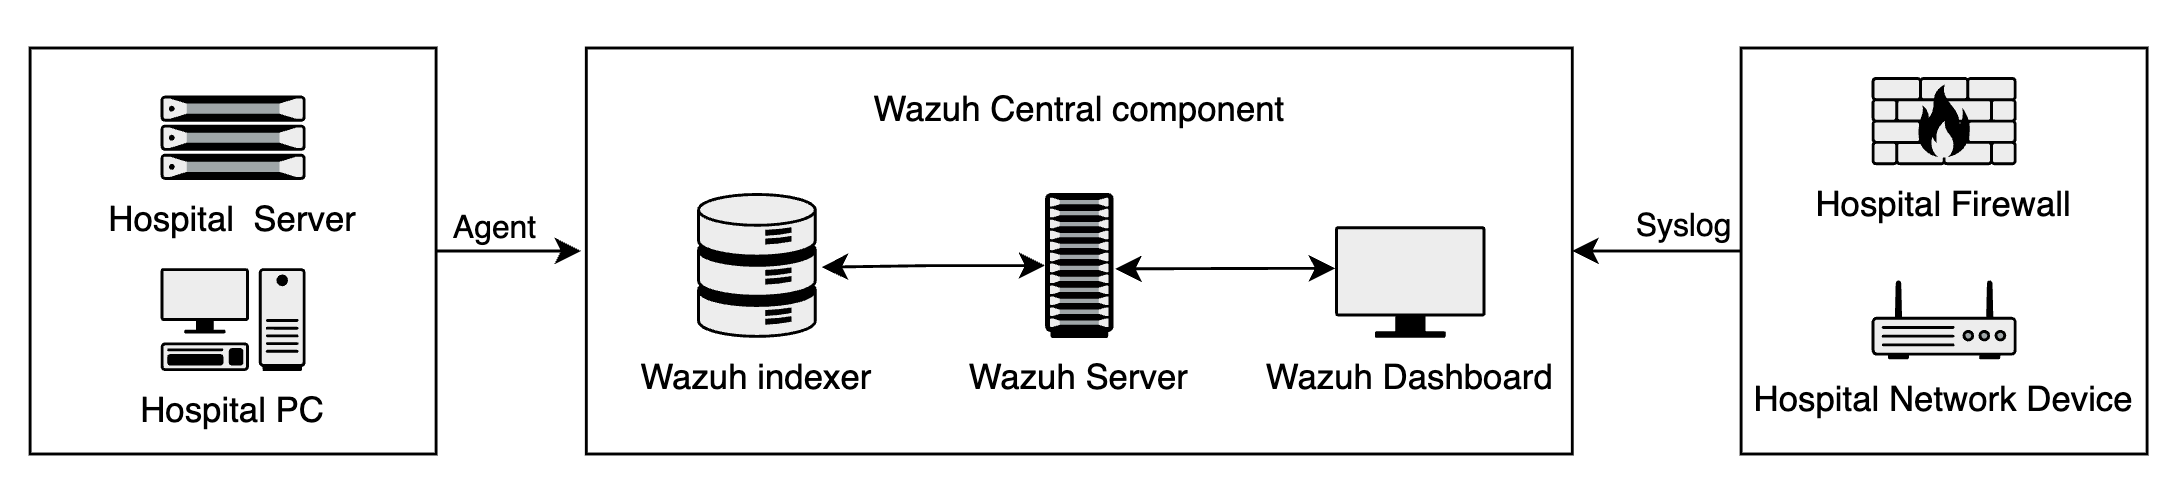
\includegraphics[width=\textwidth]{images/system_architecture.png} 
    \caption{High-Level System Architecture of the Proposed SIEM Solution.}
    \label{fig:system_architecture}
\end{figure}

\subsection{Data Collection Layer}
This foundational layer is responsible for gathering security data from a wide range of sources across the hospital's IT infrastructure. 
\begin{itemize}
    \item \textbf{Agent-based Collection:} Lightweight Wazuh agents will be deployed on endpoints such as hospital servers (e.g., Hospital Web Server) and staff PCs. These agents perform real-time log data collection, file integrity monitoring, and vulnerability detection, forwarding the data securely to the central manager.
    \item \textbf{Syslog Collection:} For network devices like firewalls and routers that cannot run a native agent, log data will be collected via the standard Syslog protocol. This ensures comprehensive visibility into network traffic and access control events.
\end{itemize}

\subsection{Processing and Analysis Layer}
The central server, referred to as the "Wazuh Central Component" in the architecture diagram, is the core of the SIEM. It processes and analyzes the raw data collected from the agents and syslog feeds.
\begin{itemize}
    \item \textbf{Wazuh Server:} This component receives the data, decodes and normalizes it, and analyzes it against a comprehensive rule set to identify security events, misconfigurations, and potential threats.
    \item \textbf{Wazuh Indexer:} The processed and enriched data is then sent to the Wazuh indexer (powered by Elasticsearch). This component indexes the data, making it highly searchable and enabling rapid querying for threat hunting and historical analysis.
\end{itemize}

\subsection{Presentation and Alerting Layer}
The user-facing layer provides the tools for security analysts to interact with the data and manage alerts.
\begin{itemize}
    \item \textbf{Wazuh Dashboard:} This web-based interface (powered by Kibana) provides a holistic view of the security environment. It offers customizable dashboards, visualizations, and reporting tools that allow analysts to monitor security events in real-time, investigate incidents, and demonstrate compliance.
\end{itemize}

% --- Section 3.2: Development Methodology ---
\section{Development Methodology}
\label{sec:dev-methodology}
The project will follow a phased, iterative development methodology. The project is divided into five distinct phases:
\begin{enumerate}
    \item \textbf{Phase 1: Environment Setup:} Configure the Proxmox virtual environment, deploying one VM for the Wazuh server and separate VMs for the Windows 11 and Ubuntu endpoints.
    \item \textbf{Phase 2: Platform Installation and Integration:} Install the latest stable version of the Wazuh platform. Integrate the chosen firewall (see Section \ref{sec:tools}) to forward syslog data.
    % NOTE: Added custom decoder development to the plan.
    \item \textbf{Phase 3: Rule and Decoder Development:} Deploy and configure agents. Develop one to two custom decoders for any unique log sources. Tune correlation rules to detect specific threats.
    \item \textbf{Phase 4: Dashboard Customization:} Design and build custom dashboards in the Wazuh Dashboard to visualize key security events from all log sources.
    \item \textbf{Phase 5: System Testing:} Execute the test cases defined in the evaluation plan (Section \ref{sec:evaluation}) to validate the system's effectiveness and document the results for Chapter 4.
\end{enumerate}


% --- Section 3.3: Tools and Technologies ---
\section{Tools and Technologies}
\label{sec:tools}
The project will leverage a combination of enterprise-grade and open-source software to build a realistic security monitoring lab.
\begin{itemize}
    \item \textbf{Virtualization Platform (Proxmox VE):} A powerful open-source virtualization platform will be used to host Wazuh and endpoint virtual machines.
     \item \textbf{SIEM Platform (Wazuh v4.12):} The project will use Wazuh version 4.12, as specified in the project proposal. It was chosen for its comprehensive, open-source security features and its flexibility in allowing custom decoder and rule development.
    \item \textbf{Endpoint Operating Systems:} To simulate a realistic environment, Wazuh agents will be tested on both \textbf{Windows 11} (representing user workstations) and \textbf{Ubuntu Server } (representing a web or database server).
    % NOTE: This is the updated firewall section with the contingency plan.
    \item \textbf{Network Firewall:} The primary goal is to integrate a physical \textbf{FortiGate firewall} as a log source to test the SIEM's ability to analyze data from an enterprise-grade device. As a contingency plan to ensure project completion in the event of access delays, an open-source \textbf{OPNsense firewall} will be configured in a virtual machine as a representative alternative for testing network log ingestion and analysis.
\end{itemize}

% --- Section 3.4: System Evaluation Plan ---
\section{System Evaluation Plan}
\label{sec:evaluation}
To validate the functionality of the implemented SIEM, a series of controlled tests will be conducted. This plan will be executed and the results analyzed in detail in Chapter 4.
\begin{itemize}
    \item \textbf{Test Case 1 (Brute-Force Attack):} A script will simulate repeated failed SSH login attempts on the Ubuntu server to test agent-based log detection.
    \item \textbf{Test Case 2 (File Integrity Monitoring):} A critical configuration file on the Windows 11 endpoint will be modified to test the FIM capabilities.
    % NOTE: Updated firewall test case to be generic.
    \item \textbf{Test Case 3 (Firewall Log Analysis):} A specific "deny" rule on the integrated firewall (FortiGate or OPNsense) will be triggered to verify syslog ingestion and alerting.
    % NOTE: Added a new test case for your custom decoder.
    \item \textbf{Test Case 4 (Custom Log Analysis):} A custom log entry will be generated on a monitored endpoint. The expected outcome is a successful parse by the custom decoder, generating a specific, readable alert in the Wazuh Dashboard.
\end{itemize}
The timely and accurate generation of an alert will determine the success of each test.



  